% 
% (c) Copyright 2016 Tabea Mendez
% 
% This source is free: you can redistribute it and/or modify
% it under the terms of the GNU General Public License as published by
% the Free Software Foundation, either version 3 of the License, or
% (at your option) any later version.
% 
% This source is distributed in the hope that it will be useful,
% but WITHOUT ANY WARRANTY; without even the implied warranty of
% MERCHANTABILITY or FITNESS FOR A PARTICULAR PURPOSE.  See the
% GNU General Public License for more details.
% 
% You should have received a copy of the GNU General Public License
% along with this source.  If not, see <http://www.gnu.org/licenses/>.
%
%%%%%%%%%%%%%%%%%%%%%%%%%%%%%%%%%%%%%%%%%%%%%%%%%%%%%%%%%%%%%%%%%%%%%%%%%%%%%%

\vspace*{-0.5cm}
\begin{minipage}{0.4\textwidth}
 $ $\\[0.5cm]
 Ein einfacher aber indirekter Weg IIR-Filter zu designen ist mittels der Bilinear-Transformation und den Design-Methoden von analogen Filtern. Dazu sind folgende schritte notwendig:
\end{minipage}
\begin{minipage}{0.05\textwidth}$ $\end{minipage}
\begin{minipage}{0.55\textwidth}
 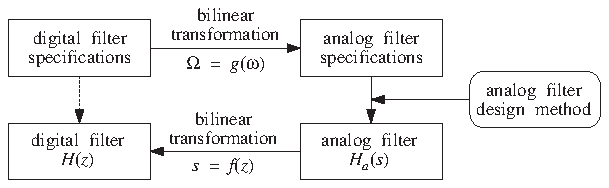
\includegraphics[width = \textwidth]{pic/IIRFilterDesign.pdf}
\end{minipage}\\
\begin{itemize}
 \item Die Spezifikationen des digitalen Frequenzganges mittels der Bilinear-Transformation in Spezifikationen des entsprechenden analogen Tiefpasses umwandeln.\\[0.1cm]
 \begin{tabular}{lclcl}
	digitaler Tiefpass &$\qquad\Rightarrow\qquad$& analoger Tiefpass:&$\quad$&
	\fcolorbox{CadetRed}{white}{$\Omega = g_{TP}(\omega) = \tan\left(\dfrac{\omega}{2}\right)$}\\[0.45cm]
	digitaler Hochpass &$\qquad\Rightarrow\qquad$& analoger Tiefpass:&$\quad$&
	\fcolorbox{CadetRed}{white}{$\Omega = g_{HP}(\omega) = -\cot\left(\dfrac{\omega}{2}\right)$}\\[0.45cm]
	digitaler Bandpass &$\qquad\Rightarrow\qquad$& analoger Tiefpass:&$\quad$&
	\fcolorbox{CadetRed}{white}{$\Omega = g_{BP}(\omega) = \dfrac{c-\cos(\omega)}{\sin(\omega)}$}\\[0.45cm]
	digitale Bandsperre &$\qquad\Rightarrow\qquad$& analoger Tiefpass:&$\quad$&
	\fcolorbox{CadetRed}{white}{$\Omega = g_{BS}(\omega) = \dfrac{\sin(\omega)}{\cos(\omega)-c}$}\\[0.45cm]
 \end{tabular}
 \item Den analogen Tiefpass $H_a(s)$ mit analogen Filter-Design-Methoden designen.
 \item Den analogen Tiefpass $H_a(s)$ mit der Bilinear-Transformation in das gewünschte digitale Filter $H(z)$ zurückmappen.\\[0.1cm]
 \begin{tabular}{lclcl}
	analoger Tiefpass&$\qquad\Rightarrow\qquad$& digitaler Tiefpass:&$\quad$&
	\fcolorbox{CadetRed}{white}{$s = f_{TP}(z) = \dfrac{1-z^{-1}}{1+z^{-1}}$}\\[0.45cm]
	analoger Tiefpass &$\qquad\Rightarrow\qquad$& digitaler Hochpass:&$\quad$&
	\fcolorbox{CadetRed}{white}{$s = f_{HP}(z) = \dfrac{1+z^{-1}}{1-z^{-1}}$}\\[0.45cm]
	analoger Tiefpass &$\qquad\Rightarrow\qquad$& digitaler Bandpass:&$\quad$&
	\fcolorbox{CadetRed}{white}{$s = f_{BP}(z) = \dfrac{1-2cz^{-1}+z^{-2}}{1-z^{-2}}$}\\[0.45cm]
	analoger Tiefpass &$\qquad\Rightarrow\qquad$& digitale Bandsperre:&$\quad$&
	\fcolorbox{CadetRed}{white}{$s = f_{BS}(z) = \dfrac{1-z^{-2}}{1-2cz^{-1}+z^{-2}}$}\\[0.45cm]
 \end{tabular}
 \item Damit gelten folgende Beziehungen zwischen dem analogen und digitalen Filter\\[0.2cm]
 \fcolorbox{CadetRed}{white}{$H(z) = H_a(s)\Big|_{s=f(z)}=H_a(f(z))$}$\qquad$\fcolorbox{CadetRed}{white}{$H(\omega) =H_a(s)\Big|_{s = j\Omega}= H_a(\Omega)\Big|_{\Omega=g(\omega)}=H_a(g(\omega))$}
\end{itemize}

\section{Eigenschaften der Bilinear-Transformation}
	Die Bilinear-Transformation mappt ...
	\begin{itemize}
		\item  die linke $s$-Halbebene auf das innere des Einheitskreises der $z$-Ebene (wenn $|c|\leq 1$).\\[0.15cm]
		\fcolorbox{CadetRed}{white}{stabiles analoges Filter$\;\stackrel{\mathrm{\begin{array}{l}\tiny{|c|\leq 1}\\[0.05cm]\end{array}}}\Leftrightarrow\;$stabiles digitales Filter}\\[-0.4cm]
		\item die analoge Frequenzachse $s=j\Omega$ auf\\ die digitale Frequenzachse $z=\e^{j\omega}$.\\[0.2cm]
		\fcolorbox{CadetRed}{white}{$\omega = \pm\pi\qquad \mathrel{\widehat=}\qquad\Omega =\pm\infty$}\\[-2.5cm]
	\end{itemize}
	\begin{minipage}{0.45\textwidth}$ $\end{minipage}
	\begin{minipage}{0.5\textwidth}
		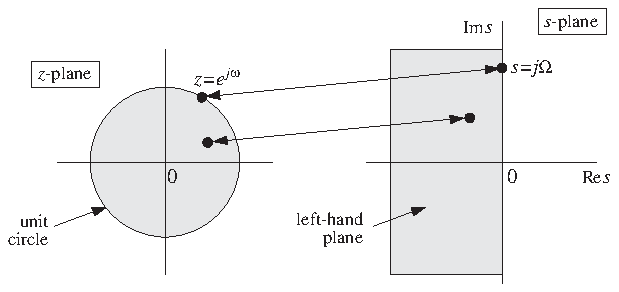
\includegraphics[width = \textwidth]{pic/bilinearTrans.pdf}
	\end{minipage}
	
\section{Tiefpass-Filter und Hochpass-Filter erster Ordnung}
	\begin{itemize}
		\item Ein digitales Filter erster Ordnung hat die parametrische Form$\qquad$\fcolorbox{CadetRed}{white}{$H(z) = \dfrac{b_0+b_1\,z^{-1}}{1+a_1\,z^{-1}}$}\\[-0.15cm]
		\item Von diesem muss die erlaubte Dämpfung $A_c$ (in $\db$) bei der Grenzfrequenz $\omega_c$ spezifiziert werden.\\[0.1cm]
		\fcolorbox{CadetRed}{white}{$\big|H(\omega_c)\big|^2 = G_c^2 = 10^{-A_c/10}$}$\qquad$\fcolorbox{CadetRed}{white}{$G_c=10^{-A_c/20}$}$\qquad$\fcolorbox{CadetRed}{white}{$A_c = -10\,\log_{10}(G_c^2)= -20\,\log_{10}(G_c)$}\\[0.15cm]
		Oft$\quad$ \fcolorbox{black}{white}{$A_c = 3\,\db\quad\Rightarrow\quad G_c^2 = 1/2$}\\[-0.5cm]
		\item Die entsprechende analoge Grenzfrequenz ist$\qquad$\fcolorbox{CadetRed}{white}{$\Omega_c = g_{LP}(\omega_c)=  \tan\left(\dfrac{\omega_c}{2}\right) = \tan\left(\dfrac{\pi f_c}{f_s}\right)$}\\[0.2cm]
	\end{itemize}
	\begin{minipage}{0.48\textwidth}
		\textbf{\large{Analoges Tiefpass-Filter}}\\[0.2cm]
		\fcolorbox{CadetRed}{white}{$H_a(s)=\dfrac{\alpha}{s+\alpha}$}\\[0.2cm]
		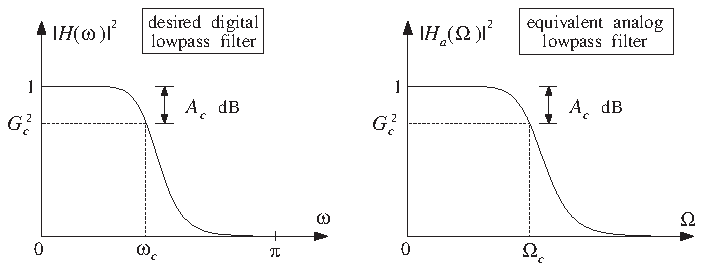
\includegraphics[width = \textwidth]{pic/TP1ordnung.pdf}\\[-0.5cm]
		\begin{itemize}
		 \item Parameter $\alpha$\\[0.1cm]
		 $\big|H_a(\Omega_c)\big|^2 = \dfrac{\alpha^2}{|j\Omega_c+\alpha|^2} = \dfrac{\alpha^2}{\Omega_c^2+\alpha^2} = G_c^2$\\[0.2cm]
		 $\Rightarrow\quad\;$\fcolorbox{CadetRed}{white}{$\alpha = \dfrac{G_c}{\sqrt{1-G_c^2}}\,\,\Omega_c = \underbrace{\dfrac{G_c}{\sqrt{1-G_c^2}}}_{1 \text{ if } G_c^2=1/2}\,\tan\left(\dfrac{\omega_c}{2}\right)$}\\[0.2cm]
		\end{itemize}
		\textbf{\large{Digitales Tiefpass-Filter}}\\[-0.25cm]
		\begin{itemize}
		 \item Übertragungsfunktion $H(z)$\\[0.05cm]
		 $H(z) = H_a(s)\Big|_{s=f_{TP}(z)}=\dfrac{\alpha\,(1+z^{-1})}{1-z^{-1}+\alpha\,(1+z^{-1})}\!\!\!\!\!\!$\\[0.25cm]
		 $\Rightarrow\quad\;$\fcolorbox{CadetRed}{white}{$H(z) = b\,\dfrac{1+z^{-1}}{1-a\,z^{-1}}$}$\quad$\\[0.2cm]
		 \textcolor{white}{$\Rightarrow\quad\quad$}mit$\quad$\fcolorbox{black}{white}{$a = \dfrac{1-\alpha}{1+\alpha},\quad b=\dfrac{\alpha}{1+\alpha}=\dfrac{1-a}{2}$}\\[0.1cm]
		 \item Frequenzgang $H(\omega)$\\[0.2cm]
		 $H(\omega) = H_a(\Omega)\Big|_{\Omega=g_{TP}(\omega)}=\dfrac{\alpha}{\alpha + j\tan(\omega/2)}$\\[0.25cm]
		 $\Rightarrow\quad\;$\fcolorbox{CadetRed}{white}{$\big|H(\omega)\big|^2 = \dfrac{\alpha^2}{\alpha^2 + \tan^2(\omega/2)}$}
		\end{itemize}
	\end{minipage}
	\begin{minipage}{0.045\textwidth}
		\begin{tabular}{c|c}
			\\[17.5cm]
		\end{tabular}
	\end{minipage}
	\begin{minipage}{0.48\textwidth}
		\textbf{\large{Analoges Hochpass-Filter}}\\[0.2cm]
		\fcolorbox{CadetRed}{white}{$H_a(s)=\dfrac{s}{s+\alpha}$}\\[0.2cm]
		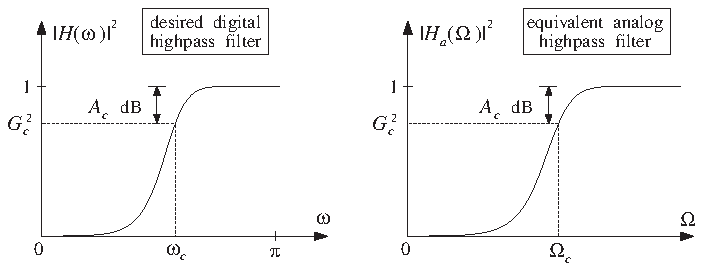
\includegraphics[width = \textwidth]{pic/HP1ordnung.pdf}\\[-0.5cm]
		\begin{itemize}
		 \item Parameter $\alpha$\\[0.1cm]
		 $\big|H_a(\Omega_c)\big|^2 = \dfrac{\Omega_c^2}{|j\Omega_c+\alpha|^2} = \dfrac{\Omega_c^2}{\Omega_c^2+\alpha^2} = G_c^2$\\[0.2cm]
		 $\Rightarrow\quad\;$\fcolorbox{CadetRed}{white}{$\alpha = \dfrac{\sqrt{1-G_c^2}}{G_c}\,\,\Omega_c = \underbrace{\dfrac{\sqrt{1-G_c^2}}{G_c}}_{1 \text{ if } G_c^2=1/2}\,\tan\left(\dfrac{\omega_c}{2}\right)$}\\[0.2cm]
		\end{itemize}
		\textbf{\large{Digitales Hochpass-Filter}}\\[-0.25cm]
		\begin{itemize}
		 \item Übertragungsfunktion $H(z)$\\[0.05cm]
		 $H(z) = H_a(s)\Big|_{s=f_{TP}(z)}=\dfrac{1-z^{-1}}{1-z^{-1}+\alpha\,(1+z^{-1})}\!\!\!\!\!\!$\\[0.25cm]
		 $\Rightarrow\quad\;$\fcolorbox{CadetRed}{white}{$H(z) = b\,\dfrac{1-z^{-1}}{1-a\,z^{-1}}$}$\quad$\\[0.2cm]
		 \textcolor{white}{$\Rightarrow\quad\quad$}mit$\quad$\fcolorbox{black}{white}{$a = \dfrac{1-\alpha}{1+\alpha},\quad b=\dfrac{1}{1+\alpha}=\dfrac{1+a}{2}$}\\[0.1cm]
		 \item Frequenzgang $H(\omega)$\\[0.2cm]
		 $H(\omega) = H_a(\Omega)\Big|_{\Omega=g_{TP}(\omega)}=\dfrac{j\tan(\omega/2)}{\alpha + j\tan(\omega/2)}$\\[0.25cm]
		 $\Rightarrow\quad\;$\fcolorbox{CadetRed}{white}{$\big|H(\omega)\big|^2 = \dfrac{\tan^2(\omega/2)}{\alpha^2 + \tan^2(\omega/2)}$}
		\end{itemize}
	\end{minipage}
	\begin{itemize}
	 \item Wenn des Hochpass- und das Tiefpass-Filter die selbe $3\,\db$-Grenzfrequenz $\omega_c$ haben, sind sie komplementäre Filter.\\[0.2cm]
	 \fcolorbox{CadetRed}{white}{$H_{TP}(z) + H_{HP}(z) = 1$}$\qquad$und$\qquad$\fcolorbox{CadetRed}{white}{$\alpha = \Omega_c = \tan\left(\dfrac{\omega_c}{2}\right)$}
	\end{itemize}
\newpage
\section{Notch-Filter und Peak-Filter zweiter Ordnung}
	\vspace*{-0.2cm}\begin{itemize}
		\item Ein digitales Filter zweiter Ordnung hat die parametrische Form$\qquad$\fcolorbox{CadetRed}{white}{$H(z) = \dfrac{b_0+b_1\,z^{-1}+b_2\,z^{-2}}{1+a_1\,z^{-1}+a_2\,z^-2}$}\\[-0.45cm]
		\item Die Spezifikations-Parameter eines Notch- bzw. Peak-Filters sind:\\[0.1cm]
		- Mittenfrequenz $\omega_0$\\[0.15cm]
		- Bandbreite \fcolorbox{CadetRed}{white}{$\Delta \omega = \omega_2-\omega_1$}\\[-0.1cm]
		- Dämpfung $G_B^2$ bei den Grenzfrequenzen $\omega_1$ und $\omega_2\quad$\fcolorbox{CadetRed}{white}{$G_B^2 = \big|H(\omega_1)\big|^2 = \big|H(\omega_2)\big|^2$}\\[-0.45cm]
		\item Die entsprechenden analogen Parameter-Spezifikationen sind:\\[0.15cm]
		\fcolorbox{CadetRed}{white}{$\Omega_0 = \tan\left(\dfrac{\omega_0}{2}\right)$}$\qquad$
		\fcolorbox{CadetRed}{white}{$\Delta\Omega = (1+\Omega_0^2)\,\tan\left(\dfrac{\Delta\omega}{2}\right)$}$\qquad$
		\fcolorbox{CadetRed}{white}{$\Omega_0^2 = \Omega_1\cdot\Omega_2$}
	\end{itemize}
	\begin{minipage}{0.48\textwidth}
		\textbf{\large{Analoges Notch-Filter}}\\[0.2cm]
		\fcolorbox{CadetRed}{white}{$H_a(s)=\dfrac{s^2 + \Omega_0^2}{s^2+\alpha s+ \Omega_0^2}$}\\[0.2cm]
		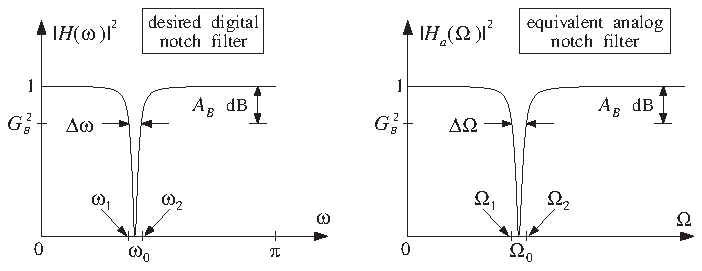
\includegraphics[width = \textwidth]{pic/Notch2ordnung.pdf}\\[-0.5cm]
		\begin{itemize}
		 \item Parameter $\alpha$\\[0.1cm]
		 $\big|H_a(\Omega_{1,2})\big|^2 = \dfrac{(\Omega_{1,2}^2-\Omega_0^2)^2}{(\Omega_{1,2}^2-\Omega_0^2)^2+\alpha^2\,\Omega_{1,2}^2} = G_B^2$\\[0.2cm]
		 $\Rightarrow\quad\;$\fcolorbox{CadetRed}{white}{$\alpha  = \underbrace{\dfrac{\sqrt{1-G_B^2}}{G_B}}_{1 \text{ if } G_B^2=1/2}\,\underbrace{(1+\Omega_0^2)\,\tan\left(\dfrac{\Delta\omega}{2}\right)}_{\Delta\Omega}$}\\[0.25cm]
		\end{itemize}
		\textbf{\large{Digitales Notch-Filter}}\\[-0.3cm]
		\begin{itemize}
		 \item Übertragungsfunktion $H(z)$\\[0.1cm]
		 $H(z) = H_a(s)\Big|_{s=f_{TP}(z)}$\\[0.2cm]
		 $\Rightarrow\quad$\fcolorbox{CadetRed}{white}{$H(z) = b\,\dfrac{1-2\cos(\omega_0)z^{-1}+z^{-2}}{1-2b\cos(\omega_0)\,z^{-1}+(2b-1)\,z^{-2}}$}$\quad$\\[0.2cm]
		 \textcolor{white}{$\Rightarrow\quad\;$}mit$\quad$\fcolorbox{black}{white}{$b=\dfrac{1}{1+\underbrace{\dfrac{\sqrt{1-G_B^2}}{G_B}\,\tan\left(\dfrac{\Delta\omega}{2}\right)}_{\beta}}$}\\[0.1cm]
		 \item Frequenzgang $H(\omega)$\\[0.2cm]
		 $H(\omega) = H_a(\Omega)\Big|_{\Omega=g_{TP}(\omega)}\\[0.2cm]
		 \hspace*{0.9cm}=\dfrac{-\tan^2(\frac{\omega}{2}) + \Omega_0^2}{-\tan^2(\frac{\omega}{2})+j\alpha\tan(\frac{\omega}{2})+ \Omega_0^2}$\\[0.25cm]
		 $\Rightarrow\quad\;$\fcolorbox{CadetRed}{white}{$\big|H(\omega)\big|^2 = \dfrac{(\tan^2(\frac{\omega}{2})-\Omega_0^2)^2}{(\tan^2(\frac{\omega}{2})-\Omega_0^2)^2+\alpha^2\,\tan^2(\frac{\omega}{2})}$}
		\end{itemize}
	\end{minipage}
	\begin{minipage}{0.045\textwidth}
		\begin{tabular}{c|c}
			\\[19.6cm]
		\end{tabular}
	\end{minipage}
	\begin{minipage}{0.48\textwidth}
		\textbf{\large{Analoges Peak-Filter}}\\[0.2cm]
		\fcolorbox{CadetRed}{white}{$H_a(s)=\dfrac{\alpha s}{s^2+\alpha s+ \Omega_0^2}$}\\[0.2cm]
		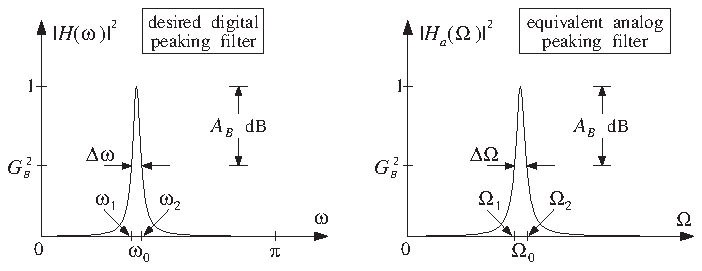
\includegraphics[width = \textwidth]{pic/Preak2ordnung.pdf}\\[-0.5cm]
		\begin{itemize}
		 \item Parameter $\alpha$\\[0.1cm]
		 $\big|H_a(\Omega_{1,2})\big|^2 = \dfrac{\alpha^2\,\Omega_{1,2}^2}{(\Omega_{1,2}^2-\Omega_0^2)^2+\alpha^2\,\Omega_{1,2}^2} = G_B^2$\\[0.2cm]
		 $\Rightarrow\quad\;$\fcolorbox{CadetRed}{white}{$\alpha = \underbrace{\dfrac{G_B}{\sqrt{1-G_B^2}}}_{1 \text{ if } G_B^2=1/2}\,\underbrace{(1+\Omega_0^2)\,\tan\left(\dfrac{\Delta\omega}{2}\right)}_{\Delta\Omega}$}\\[0.25cm]
		\end{itemize}
		\textbf{\large{Digitales Peak-Filter}}\\[-0.3cm]
		\begin{itemize}
		 \item Übertragungsfunktion $H(z)$\\[0.1cm]
		 $H(z) = H_a(s)\Big|_{s=f_{TP}(z)}$\\[0.2cm]
		 $\Rightarrow\quad$\fcolorbox{CadetRed}{white}{$H(z) = \dfrac{(1-b)\,(1-z^{-2})}{1-2b\cos(\omega_0)\,z^{-1}+(2b-1)\,z^{-2}}$}$\quad$\\[0.2cm]
		 \textcolor{white}{$\Rightarrow\quad\;$}mit$\quad$\fcolorbox{black}{white}{$b=\dfrac{1}{1+\underbrace{\dfrac{G_B}{\sqrt{1-G_B^2}}\,\tan\left(\dfrac{\Delta\omega}{2}\right)}_{\beta}}$}\\[0.1cm]
		 \item Frequenzgang $H(\omega)$\\[0.2cm]
		 $H(\omega) = H_a(\Omega)\Big|_{\Omega=g_{TP}(\omega)}\\[0.2cm]
		 \hspace*{0.9cm}=\dfrac{j\alpha\tan(\frac{\omega}{2})}{-\tan^2(\frac{\omega}{2})+j\alpha\tan(\frac{\omega}{2})+ \Omega_0^2}$\\[0.25cm]
		 $\Rightarrow\quad\;$\fcolorbox{CadetRed}{white}{$\big|H(\omega)\big|^2 = \dfrac{\alpha^2\,\tan^2(\frac{\omega}{2})}{(\tan^2(\frac{\omega}{2})-\Omega_0^2)^2+\alpha^2\,\tan^2(\frac{\omega}{2})}$}
		\end{itemize}
	\end{minipage}
\newpage

	\begin{itemize}
	 \item Das Notch-Filter hat eine Doppelte Nullstelle bei $\omega_0\quad$  \fcolorbox{CadetRed}{white}{$z_{NS} = \e^{\pm j\omega_0}$}\\
	 und das Peak-Filter hat die Nullstellen Nullstellen bei DC und bei der halben Abtast-frequenz$\quad$\fcolorbox{CadetRed}{white}{$z_{NS} = \pm 1$}
	 \item Wenn des Notch- und das Peak-Filter die selbe $3\,\db$-Mittenfrequenz $\omega_0$ und die selbe Bandbreite $\Delta\omega$ haben, sind sie komplementäre Filter. %\\[0.2cm]
	 $\quad$\fcolorbox{CadetRed}{white}{$H_{notch}(z) + H_{peak}(z) = 1$}
	\end{itemize}

	\section{Filter höherer Ordnung}
		\begin{itemize}
			\item Für das Design eines Filters höherer Ordnung müssen folgende Spezifikationen bekannt sein:\\[0.2cm]
			\begin{minipage}{0.35\textwidth}
			 \begin{itemize}
			  \item Filtertyp
			  \item Durchlassbereich $f_{pass}$
			  \item Sperrbereich $f_{stop}$
			 \end{itemize}
			\end{minipage}
			\begin{minipage}{0.5\textwidth}
			 \begin{itemize}
			  \item Passband-Dämpfung $A_{pass}$
			  \item Stoppband-Dämpfung $A_{stop}$
			 \end{itemize}
			\end{minipage}
			\item Die Pass- und Stoppband-Dämpfung können in relativen ($\db$) oder in Absoluten Werten gegeben sein.\\[0.2cm]
			\fcolorbox{CadetRed}{white}{$\begin{array}{lcl}\varepsilon_{pass}& =& \sqrt{10^{A_{pass}/10}-1}\\[0.2cm]\varepsilon_{stop}&=&\sqrt{10^{A_{stop}/10}-1}\end{array}$}$\qquad\Leftrightarrow\qquad$\fcolorbox{CadetRed}{white}{$\begin{array}{lcl}A_{pass}&=&10\log_{10}(1+\varepsilon_{pass}^2)\\[0.2cm]A_{stop}&=&10\log_{10}(1+\varepsilon_{stop}^2)\end{array}$}\\[-0.075cm]
			\item Umrechnung der digitalen Filter-Spezifikationen in die Spezifikationen des analogen Tiefpasses mittels Bilinear-Transformationen.
		\end{itemize}

		\begin{tabularx}{\textwidth}{>{\centering\arraybackslash}X|>{\centering\arraybackslash}X}
			\textbf{Tiefpass} & \textbf{Hochpass}\\[0.1cm]
			\hline&\\[-0.3cm]
			$\begin{array}{l}\text{\fcolorbox{CadetRed}{white}{$\Omega_{pass} = \tan\left(\dfrac{\omega_{pass}}{2}\right) = \tan\left(\dfrac{\pi f_{pass}}{f_s}\right)$}}\\[0.55cm]
			\text{\fcolorbox{CadetRed}{white}{$\Omega_{stop} = \tan\left(\dfrac{\omega_{stop}}{2}\right) = \tan\left(\dfrac{\pi f_{stop}}{f_s}\right)$}}\end{array}$
			& 
			$\begin{array}{l}\text{\fcolorbox{CadetRed}{white}{$\Omega_{pass} = -\cot\left(\dfrac{\omega_{pass}}{2}\right) = -\cot\left(\dfrac{\pi f_{pass}}{f_s}\right)$}}\\[0.55cm]
			\text{\fcolorbox{CadetRed}{white}{$\Omega_{stop} = -\cot\left(\dfrac{\omega_{stop}}{2}\right) = -\cot\left(\dfrac{\pi f_{stop}}{f_s}\right)$}}\end{array}$\\[1.3cm]
			\hspace*{-0.5cm}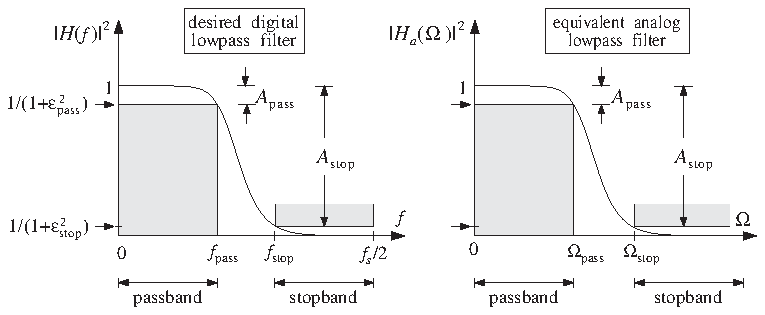
\includegraphics[width = 0.5\textwidth]{pic/ButterworthTP.pdf}
			& 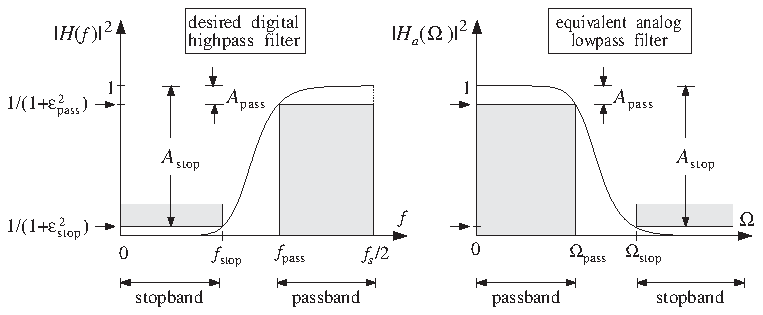
\includegraphics[width = 0.5\textwidth]{pic/ButterworthHP.pdf}\\
			\hline&\\[-0.3cm]
			\textbf{Bandpass} & \textbf{Bandsperre}\\[0.1cm]
			\hline&\\[-0.3cm]
			$\begin{array}{c}\text{\fcolorbox{black}{white}{$c = \cos(\omega_c)$}$\quad\Rightarrow\quad$
			\fcolorbox{CadetRed}{white}{$c = \dfrac{\sin(\omega_{pa}+\omega_{pb})}{\sin(\omega_{pa}) + \sin(\omega_{pb})}$}}\\[0.55cm]
			\text{\fcolorbox{CadetRed}{white}{$\Omega_{pass} = \left|\dfrac{c-\cos(\omega_{pb})}{\sin(\omega_{pb})}\right|$}}\\[0.6cm]
			\text{\fcolorbox{CadetRed}{white}{$\Omega_{stop} = \min\{|\Omega_{sa}|,|\Omega_{sb}|\}$}}\\[0.35cm]
			\text{mit$\quad$\fcolorbox{black}{white}{$\Omega_{sa} = \dfrac{c-\cos(\omega_{sa})}{\sin(\omega_{sa})}$}$\quad$\fcolorbox{black}{white}{$\Omega_{sb} = \dfrac{c-\cos(\omega_{sb})}{\sin(\omega_{sb})}$}}\end{array}$
			& 
			$\begin{array}{c}\text{\fcolorbox{black}{white}{$c = \cos(\omega_c)$}$\quad\Rightarrow\quad$
			\fcolorbox{CadetRed}{white}{$c = \dfrac{\sin(\omega_{pa}+\omega_{pb})}{\sin(\omega_{pa}) + \sin(\omega_{pb})}$}}\\[0.55cm]
			\text{\fcolorbox{CadetRed}{white}{$\Omega_{pass} = \left|\dfrac{\sin(\omega_{pb})}{\cos(\omega_{pb})-c}\right|$}}\\[0.6cm]
			\text{\fcolorbox{CadetRed}{white}{$\Omega_{stop} = \min\{|\Omega_{sa}|,|\Omega_{sb}|\}$}}\\[0.35cm]
			\text{mit$\quad$\fcolorbox{black}{white}{$\Omega_{sa} = \dfrac{\sin(\omega_{sa})}{\cos(\omega_{sa})-c}$}$\quad$\fcolorbox{black}{white}{$\Omega_{sb} = \dfrac{\sin(\omega_{sb})}{\cos(\omega_{sb})-c}$}}\end{array}$\\[2.5cm]
			\hspace*{-0.5cm}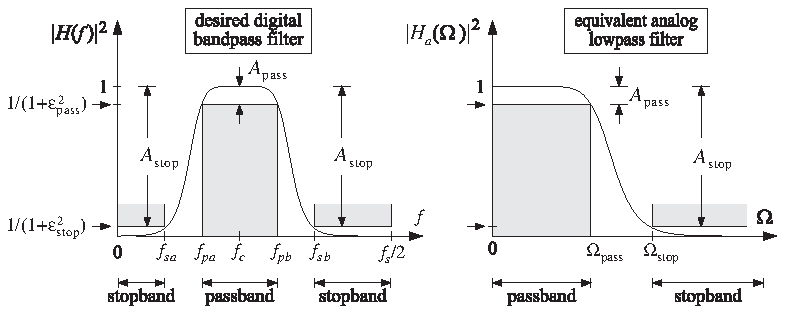
\includegraphics[width = 0.5\textwidth]{pic/ButterworthBP.pdf}
			& 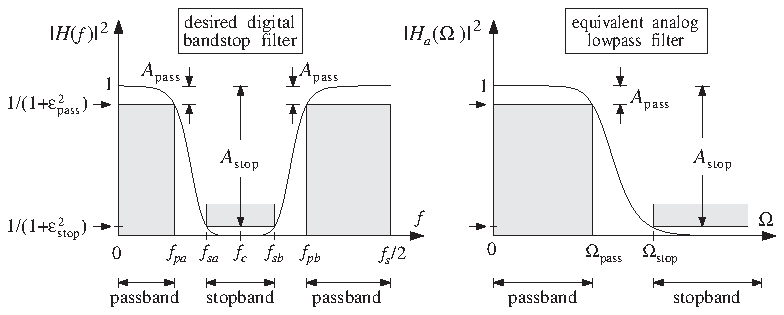
\includegraphics[width = 0.5\textwidth]{pic/ButterworthBS.pdf}\\
			\hline
		\end{tabularx}
\newpage
		\subsection{Butterworth-Filter}
			\begin{itemize}
			 \item Das analoge Tiefpass kann mit einer beliebigen Filter approximiert werden. Eine sehr weit verbreitete und simple Approximation ist das Butterworth-Filter.\\[0cm]
			 Butterworth-Filter:$\qquad$\fcolorbox{CadetRed}{white}{$\big|H(\Omega)\big|^2 = \dfrac{1}{1+\left(\dfrac{\Omega}{\Omega_0}\right)^{2N}}$}$\qquad\begin{array}{ll}\\[0.2cm]N:&\text{ Filterordnung}\\\Omega_0:&\text{ $3\,\db$ Grenzfrequenz}\end{array}$\\[0.2cm]
			 Dämpfung in $\db$:$\qquad\;\;\;$\fcolorbox{CadetRed}{white}{$A(\Omega) = -10\log_{10}\big|H(\Omega)\big|^2 = 10\log_{10}\left[1+\left(\dfrac{\Omega}{\Omega_0}\right)^{2N}\right]$}\\[-0.1cm]
			 \item Vom Butterworth-Filter ist die Ordnung $N$ zu berechnen.\\[0.075cm]
			 \fcolorbox{CadetRed}{white}{$N = \lceil N_{exakt}\rceil$}$\qquad$
			 \fcolorbox{CadetRed}{white}{$N_{exakt} = \dfrac{\ln(\varepsilon_{stop}/\varepsilon_{pass})}{\ln(\Omega_{stop}/\Omega_{pass})} = \dfrac{\ln(e)}{\ln(w)}$}$\qquad$\fcolorbox{CadetRed}{white}{$e = \dfrac{\varepsilon_{stop}}{\varepsilon_{pass}} = \sqrt{\dfrac{10^{A_{stop}/10}-1}{10^{A_{pass}/10}-1}},\quad w = \dfrac{\Omega_{stop}}{\Omega_{pass}}$}\\[-0.1cm]
			 \item Aufgrund der aufgerundeten Ordnung $N$ ist das Filter etwas ''zu gut'', d.h. dass entweder die Stoppband-Dämpfung oder die Passband-Dämpfung ''zu gut'' ist, je nach dem wie die exakte $3\,\db$ Grenzfrequenz $\Omega_0$ bestimmt wird.\\
			 $A(\Omega_{stop})>A_{stop}:\qquad\;$\fcolorbox{CadetRed}{white}{$\Omega_0 = \dfrac{\Omega_{pass}}{(10^{A_{pass}/10}-1)^{1/2N}} = \dfrac{\Omega_{pass}}{\varepsilon_{pass}^{1/N}}$}$\qquad$\\[0.2cm]
			 $A(\Omega_{pass})<A_{pass}:\qquad$\fcolorbox{CadetRed}{white}{$\Omega_0 = \dfrac{\Omega_{stop}}{(10^{A_{stop}/10}-1)^{1/2N}} = \dfrac{\Omega_{stop}}{\varepsilon_{stop}^{1/N}}$}\\
			 \item Die Übertragungsfunktion $H(s)$ kann über eine spektrale Faktorisierung ermittelt werden. Daraus geht hervor, dass alle Polstellen $s_i$ (Nullstellen des Nenner-Polynoms) auf einem Halbkreis in der linken $s$-Halbebene liegen müssen, damit das Filter stabil ist.\\[0.2cm]
			 \fcolorbox{CadetRed}{white}{$s_i = \Omega_0\,\e^{j\theta_i},\qquad \theta_i = \dfrac{\pi}{2N}(N-1+2i)$}$\qquad i=1,2,...,N$\\[0.2cm]
			 $\quad\Rightarrow\qquad$\fcolorbox{CadetRed}{white}{$H_a(s) = \myprod{i=1}{N}{\dfrac{1}{(1- \frac{1}{\Omega_0}\,\e^{-j\theta_i}\,s)}}$}\\[-3cm]
			 \hspace*{11cm}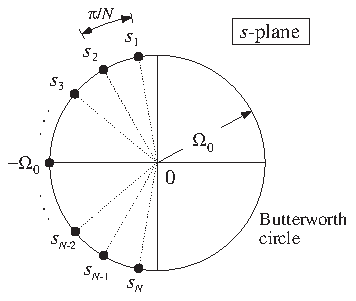
\includegraphics[width = 0.3\textwidth]{pic/ButterworthKreis.pdf}\\[-0.7cm]
			 \item Die Polstellen kommen immer in konjugiert-komplexen-Paaren vor und können daher zu Second-Order-Sections zusammengefasst werden\\[0.2cm]
			 \fcolorbox{CadetRed}{white}{$H_a(s) = H_0(s)\,H_1(s)\,H_2(s)\dots H_K(s)$}\\[0.2cm]\fcolorbox{CadetRed}{white}{$\begin{array}{lcl}H_0(s)& = &\begin{cases}\;\;\;\;\;\;1,&N=2K\\\dfrac{1}{1+s/\Omega_0},&N=2K+1\end{cases} \\[0.7cm] H_i(s) &=& \dfrac{1}{1-2\dfrac{s}{\Omega_0}\cos(\theta_i)+\dfrac{s^2}{\Omega_0^2}}\qquad i=1,2,...,K\end{array}$}\\[-0.1cm]
			 \item Der analoge Tiefpass $H_a(s)$ muss nun mit der entsprechenden Bilinear-Transformation wieder in das gewünschte digitale Filter $H(z)$ zurückgemappt werden.\\[0.1cm]
			 \begin{minipage}{0.45\textwidth}
				\begin{itemize}
				 \item Tiefpass$\qquad\overset{s=f_{TP}(z)}{\Longrightarrow}\qquad$Tiefpass\\[-0.3cm]
				 \item Tiefpass$\qquad\overset{s=f_{HP}(z)}{\Longrightarrow}\qquad$Hochpass
				\end{itemize}
			 \end{minipage}
			 \begin{minipage}{0.5\textwidth}
				\begin{itemize}
				 \item Tiefpass$\qquad\overset{s=f_{BP}(z)}{\Longrightarrow}\qquad$Bandpass\\[-0.3cm]
				 \item Tiefpass$\qquad\overset{s=f_{BS}(z)}{\Longrightarrow}\qquad$Bandsperre
				\end{itemize}
			 \end{minipage}
			\end{itemize}
\newpage
$ $\\
			\begin{tabularx}{\textwidth}{lX|lX}
			\multicolumn{2}{c|}{\textbf{\large Tiefpass}} & \multicolumn{2}{c}{\textbf{\large Hochpass}}\\[0.1cm]
			\hline&&&\\[-0.3cm]
				\multicolumn{2}{l|}{\textbf{Übertragungsfunktion $H(z)$:}} & \multicolumn{2}{l}{\textbf{Übertragungsfunktion $H(z)$:}} \\[0.15cm]
				&$H_i(z) = H_i(s)\Big|_{s=f_{TP}(z)}$ &
				&$H_i(z) = H_i(s)\Big|_{s=f_{HP}(z)}$ \\[0.4cm]
				$\Rightarrow$&\fcolorbox{CadetRed}{white}{$H_0(z) = \dfrac{G_0(1+z^{-1})}{1+a_{01}\,z^{-1}}$}&
				$\Rightarrow$&\fcolorbox{CadetRed}{white}{$H_0(z) = \dfrac{G_0(1-z^{-1})}{1+a_{01}\,z^{-1}}$}\\[0.5cm]
				&mit$\quad$\fcolorbox{black}{white}{$G_0 = \dfrac{\Omega_0}{\Omega_0+1}$}$\quad$und$\quad$\fcolorbox{black}{white}{$a_{01} = \dfrac{\Omega_0-1}{\Omega_0+1}$} &&
				mit$\quad$\fcolorbox{black}{white}{$G_0 = \dfrac{\Omega_0}{\Omega_0+1}$}$\quad$und$\quad$\fcolorbox{black}{white}{$a_{01} = -\dfrac{\Omega_0-1}{\Omega_0+1}$}\\[0.6cm]
				$\Rightarrow$&\fcolorbox{CadetRed}{white}{$H_i(z) = \dfrac{G_i(1+z^{-1})^2}{1+a_{i1}\,z^{-1}+ a_{i2}\,z^{-2}}$}&
				$\Rightarrow$&\fcolorbox{CadetRed}{white}{$H_i(z) = \dfrac{G_i(1-z^{-1})^2}{1+a_{i1}\,z^{-1}+ a_{i2}\,z^{-2}}$}\\[0.5cm]
				&mit$\,\quad$\fcolorbox{black}{white}{$G_i = \dfrac{\Omega_0^2}{1-2\,\Omega_0\cos(\theta_i)+\Omega_0^2}$}$\quad$&&
				mit$\,\quad$\fcolorbox{black}{white}{$G_i = \dfrac{\Omega_0^2}{1-2\,\Omega_0\cos(\theta_i)+\Omega_0^2}$}$\quad$\\[0.5cm]
				&und$\quad$\fcolorbox{black}{white}{$a_{i1} = \dfrac{2(\Omega_0^2-1)}{1-2\,\Omega_0\cos(\theta_i)+\Omega_0^2}$} &&
				und$\quad$\fcolorbox{black}{white}{$a_{i1} = -\dfrac{2(\Omega_0^2-1)}{1-2\,\Omega_0\cos(\theta_i)+\Omega_0^2}$}\\[0.5cm]
				&und$\quad$\fcolorbox{black}{white}{$a_{i2} = \dfrac{1+2\,\Omega_0\cos(\theta_i)+\Omega_0^2}{1-2\,\Omega_0\cos(\theta_i)+\Omega_0^2}$} &&
				und$\quad$\fcolorbox{black}{white}{$a_{i2} = \dfrac{1+2\,\Omega_0\cos(\theta_i)+\Omega_0^2}{1-2\,\Omega_0\cos(\theta_i)+\Omega_0^2}$}\\[0.6cm]
				$\Rightarrow$&\fcolorbox{CadetRed}{white}{$H(z) = H_0(z)\,H_1(z)\,H_2(z)\dots H_K(z)$}&
				$\Rightarrow$&\fcolorbox{CadetRed}{white}{$H(z) = H_0(z)\,H_1(z)\,H_2(z)\dots H_K(z)$}\\[0.5cm]
				\multicolumn{2}{l|}{\textbf{Frequenzgang $H(\omega)$:}} & \multicolumn{2}{l}{\textbf{Frequenzgang $H(\omega)$:}} \\[0.15cm]
				&$H(\omega) = H_a(\Omega)\Big|_{\Omega=g_{TP}(\omega)}$ & & $H(\omega) = H_a(\Omega)\Big|_{\Omega=g_{HP}(\omega)}$\\[0.4cm]
				$\Rightarrow$&\fcolorbox{CadetRed}{white}{$\big|H(\omega)\big|^2 = \dfrac{1}{1+(\tan(\frac{\omega}{2})/\Omega_0)^{2N}}$}&
				$\Rightarrow$&\fcolorbox{CadetRed}{white}{$\big|H(\omega)\big|^2 = \dfrac{1}{1+(\cot(\frac{\omega}{2})/\Omega_0)^{2N}}$}\\[0.8cm]
				\multicolumn{2}{l|}{\textbf{3$\,\db$ Grenzfrequenz $\omega_0$:}} & \multicolumn{2}{l}{\textbf{3$\,\db$ Grenzfrequenz $\omega_0$:}} \\[0.15cm]
				&\fcolorbox{CadetRed}{white}{$\omega_0 = 2\,\arctan(\Omega_0)$}$\quad$\fcolorbox{CadetRed}{white}{$f_0 = \dfrac{f_s}{\pi}\,\arctan(\Omega_0)$}&&\fcolorbox{CadetRed}{white}{$\omega_0 = 2\,\arctan\left(\dfrac{1}{\Omega_0}\right)$}$\quad$\fcolorbox{CadetRed}{white}{$f_0 = \dfrac{f_s}{\pi}\,\arctan\left(\dfrac{1}{\Omega_0}\right)$}\\[0.7cm]
				\hline
			\end{tabularx}
\newpage
$ $\\
			\begin{tabularx}{\textwidth}{lX|lX}			
				\multicolumn{2}{c|}{\textbf{\large Bandpass}} & \multicolumn{2}{c}{\textbf{\large Bandsperre}}\\[0.1cm]
			\hline&&&\\[-0.3cm]
				\multicolumn{2}{l|}{\textbf{Übertragungsfunktion $H(z)$:}} & \multicolumn{2}{l}{\textbf{Übertragungsfunktion $H(z)$:}} \\[0.15cm]
				&$H_i(z) = H_i(s)\Big|_{s=f_{BP}(z)}$ &
				&$H_i(z) = H_i(s)\Big|_{s=f_{BS}(z)}$ \\[0.4cm]
				$\Rightarrow$&\fcolorbox{CadetRed}{white}{$H_0(z) = \dfrac{G_0(1-z^{-2})}{1+a_{01}\,z^{-1}+a_{02}\,z^{-2}}$}&
				$\Rightarrow$&\fcolorbox{CadetRed}{white}{$H_0(z) = \dfrac{G_0(1-2c\,z^{-1}+z^{-2})}{1+a_{01}\,z^{-1}+a_{02}\,z^{-2}}$}\\[0.5cm]
				&mit$\quad$\fcolorbox{black}{white}{$G_0 = \dfrac{\Omega_0}{1+\Omega_0}$}$\quad$und$\quad$\fcolorbox{black}{white}{$a_{01} = -\dfrac{2c}{1+\Omega_0}$} &&
				mit$\quad$\fcolorbox{black}{white}{$G_0 = \dfrac{\Omega_0}{1+\Omega_0}$}$\quad$und$\quad$\fcolorbox{black}{white}{$a_{01} = -\dfrac{2c\,\Omega_0}{1+\Omega_0}$}\\[0.6cm]
				&und$\quad$\fcolorbox{black}{white}{$a_{02} = \dfrac{1-\Omega_0}{1+\Omega_0}$} &&
				und$\quad$\fcolorbox{black}{white}{$a_{02} = -\dfrac{1-\Omega_0}{1+\Omega_0}$}\\[0.6cm]
				$\Rightarrow$&\fcolorbox{CadetRed}{white}{$H_i(z)\! =\! \dfrac{G_i(1-z^{-2})^2}{1+a_{i1}z^{-1}+ a_{i2}z^{-2}+ a_{i3}z^{-3}+ a_{i4}z^{-4}}$}&
				$\Rightarrow$&\fcolorbox{CadetRed}{white}{$H_i(z)\! =\! \dfrac{G_i(1-2c\,z^{-1}+z^{-2})^2}{1+a_{i1}z^{-1}+ a_{i2}z^{-2}+ a_{i3}z^{-3}+ a_{i4}z^{-4}}$}\\[0.5cm]
				&mit$\,\quad$\fcolorbox{black}{white}{$G_i = \dfrac{\Omega_0^2}{1-2\,\Omega_0\cos(\theta_i)+\Omega_0^2}$}$\quad$&&
				mit$\,\quad$\fcolorbox{black}{white}{$G_i = \dfrac{\Omega_0^2}{1-2\,\Omega_0\cos(\theta_i)+\Omega_0^2}$}\\[0.5cm]
				&und$\quad$\fcolorbox{black}{white}{$a_{i1} = \dfrac{4c\,(\Omega_0\cos(\theta_i)-1)}{1-2\,\Omega_0\cos(\theta_i)+\Omega_0^2}$} &&
				und$\quad$\fcolorbox{black}{white}{$a_{i1} = \dfrac{4c\,\Omega_0\,(\cos(\theta_i)-\Omega_0)}{1-2\,\Omega_0\cos(\theta_i)+\Omega_0^2}$}\\[0.5cm]
				&und$\quad$\fcolorbox{black}{white}{$a_{i2} = \dfrac{2\,(2c^2+1-\Omega_0^2)}{1-2\,\Omega_0\cos(\theta_i)+\Omega_0^2}$} &&
				und$\quad$\fcolorbox{black}{white}{$a_{i2} = \dfrac{2\,(2c^2\,\Omega_0^2+\Omega_0^2-1)}{1-2\,\Omega_0\cos(\theta_i)+\Omega_0^2}$}\\[0.5cm]
				&und$\quad$\fcolorbox{black}{white}{$a_{i3} = -\dfrac{4c\,(\Omega_0\cos(\theta_i)+1)}{1-2\,\Omega_0\cos(\theta_i)+\Omega_0^2}$} &&
				und$\quad$\fcolorbox{black}{white}{$a_{i3} = -\dfrac{4c\,\Omega_0\,(\cos(\theta_i)+\Omega_0)}{1-2\,\Omega_0\cos(\theta_i)+\Omega_0^2}$}\\[0.5cm]
				&und$\quad$\fcolorbox{black}{white}{$a_{i4} = \dfrac{1+2\,\Omega_0\cos(\theta_i)+\Omega_0^2}{1-2\,\Omega_0\cos(\theta_i)+\Omega_0^2}$} &&
				und$\quad$\fcolorbox{black}{white}{$a_{i4} = \dfrac{1+2\,\Omega_0\cos(\theta_i)+\Omega_0^2}{1-2\,\Omega_0\cos(\theta_i)+\Omega_0^2}$}\\[0.6cm]
				$\Rightarrow$&\fcolorbox{CadetRed}{white}{$H(z) = H_0(z)\,H_1(z)\,H_2(z)\dots H_K(z)$}&
				$\Rightarrow$&\fcolorbox{CadetRed}{white}{$H(z) = H_0(z)\,H_1(z)\,H_2(z)\dots H_K(z)$}\\[0.5cm]
				\multicolumn{2}{l|}{\textbf{Frequenzgang $H(\omega)$:}} & \multicolumn{2}{l}{\textbf{Frequenzgang $H(\omega)$:}} \\[0.15cm]
				&$H(\omega) = H_a(\Omega)\Big|_{\Omega=g_{BP}(\omega)}$ & &$H(\omega) = H_a(\Omega)\Big|_{\Omega=g_{BS}(\omega)}$\\[0.4cm]
				$\Rightarrow$&\fcolorbox{CadetRed}{white}{$\big|H(\omega)\big|^2 = \dfrac{1}{1+\left(\dfrac{(c-\cos(\omega))/\sin(\omega)}{\Omega_0}\right)^{2N}}$}&
				$\Rightarrow$&\fcolorbox{CadetRed}{white}{$\big|H(\omega)\big|^2 = \dfrac{1}{1+\left(\dfrac{\sin(\omega)/(\cos(\omega)-c)}{\Omega_0}\right)^{2N}}$}\\[1.4cm]
				\multicolumn{2}{l|}{\textbf{3$\,\db$ Grenzfrequenzen $\omega_{0a}$ und $\omega_{0b}$:}} & \multicolumn{2}{l}{\textbf{3$\,\db$ Grenzfrequenzen $\omega_{0a}$ und $\omega_{0b}$:}} \\[0.15cm]
				&\fcolorbox{CadetRed}{white}{$\tan\!\left(\dfrac{\omega_{0a}}{2}\right) \!=\! \tan\!\left(\dfrac{\pi f_{0a}}{f_s}\right) \!=\! \dfrac{\sqrt{\Omega_0^2+1-c^2}-\Omega_0}{1+c}$}&&
				\fcolorbox{CadetRed}{white}{$\tan\!\left(\dfrac{\omega_{0a}}{2}\right) \!=\! \tan\!\left(\dfrac{\pi f_{0a}}{f_s}\right) \!=\! \dfrac{\sqrt{1+\Omega_0^2\,(1-c^2)}-1}{\Omega_0(1+c)}$}\\[0.6cm]
				&\fcolorbox{CadetRed}{white}{$\tan\!\left(\dfrac{\omega_{0b}}{2}\right) \!=\! \tan\!\left(\dfrac{\pi f_{0b}}{f_s}\right) \!=\! \dfrac{\sqrt{\Omega_0^2+1-c^2}+\Omega_0}{1+c}$}&&
				\fcolorbox{CadetRed}{white}{$\tan\!\left(\dfrac{\omega_{0b}}{2}\right) \!=\! \tan\!\left(\dfrac{\pi f_{0b}}{f_s}\right) \!=\! \dfrac{\sqrt{1+\Omega_0^2\,(1-c^2)}+1}{\Omega_0(1+c)}$}\\[0.7cm]
			\hline
			\end{tabularx}